% !TEX TS-program = xelatex
%
\documentclass{report}

  \usepackage[english]{babel}
  \usepackage{parskip}

  \usepackage{enumitem}

  \usepackage{amssymb}
  \usepackage{listings}

  \usepackage{tkz-graph}
  \tikzset{vertex/.style = {shape=circle,draw,minimum size=1}}
  \tikzset{edge/.style = {->,> = latex'}}

  \title{Process Calculi for Concurrency}
  \author{Markus Reiter, Michael Kaltschmid}

  \begin{document}
  \maketitle
  \tableofcontents

  \section{Introduction}
  This report is about $mCRL2$, a rather modern Process Calculi. We will discuss $mCRL2$ itself and concepts which are the base of it.
  \subsection{What is a Process Calculus?}
  A Process Calculus is basically an approach for formally modelling concurrent systems.
  Furthermore it is a tool for high-level description of interactions, communications and synchronizations between processes. \\
  It also provides algebraic laws to allow analyzing and transforming process descriptions and permits formal reasoning about equivalences between processes (e.g., using bisimulation) \\

  \subsection{Focus}
  There are various other forms of Process Calculi like $ACP$, $CCS$, $CSP$, $Join-Calculus$, $\mu-Calculus$, $PEPA$ or $\pi-Calculus$. However we are only going to focus on $ACP$ and $\mu-Calculus$. Specifically on $\mu-Calculus$ since it the core concept of $mCRL2$.

  \section{Labelled Transition Systems}
  A LTS is a directed labelled graph and it consists of a set of state and a set of transitoins labelled with actions that connect the states. Additionally it must have an initial state. It is also important to note that it will deadlock if a reachable state does not terminate and has no outgoing
  transitions. If a state has more than one outgoing transition with the same label to different states, then it is nondeterministic. \\[12pt]
  A LTS is a tuple $(S, A, \to,s_0>)$ where: \\

  \begin{itemize}
    \item $S$ is a set of states \\
    \item $A$ is a set of actions \\
    \item $\to\ \subseteq S \times A \times S$ is a transition relation \\
    \item $s_0 \in S$ is the initial state \\
  \end{itemize}

  \begin{tabular}{cc}
    \begin{minipage}{.5\linewidth}
      \centering
      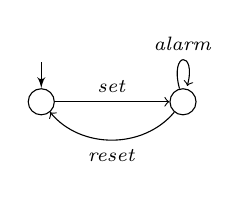
\begin{tikzpicture}[font=\sffamily\scriptsize]
        \node[vertex] (a) at (0, 0) {};
        \node[vertex] (b) at (1.8, 0) {};

        \draw[edge] (0, 0.5) to (a);
        \path[->] (a) edge  node[above] {$\mathit{set}$} (b);
        \path[->] (b) edge  [loop above] node {$\mathit{alarm}$} ();
        \path[->] (b) edge  [bend left=50] node[below] {$\mathit{reset}$} (a);
      \end{tikzpicture}
    \end{minipage}
    \begin{minipage}{.5\linewidth}
      \centering
      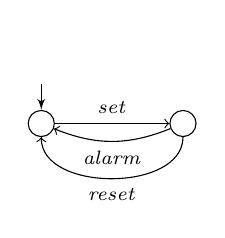
\begin{tikzpicture}[font=\sffamily\scriptsize]
        \node[vertex] (a) at (0, 0) {};
        \node[vertex] (b) at (1.8, 0) {};
        \node at (0, 1.1) {};

        \draw[edge] (0, 0.5) to (a);
        \path[->] (a) edge  node[above] {$\mathit{set}$} (b);
        \path[->] (b) edge  [bend left=22] node[below] {$\mathit{alarm}$} (a);
        \path[->] (b) edge  [bend left=90] node[below] {$\mathit{reset}$} (a);
      \end{tikzpicture}
    \end{minipage}
  \end{tabular} \\[12pt]

  In the two figures above you can see examples of two LTSs for alarm clocks. The first alarm clock on the left allows for repeated alarms which can be seen by the loop on top of the alarm state. With the second alarm clock it is only possible to signal the alarm once. \\
  Both LTSs are determistic since no state has more than one outgoing transition with the same label to a different state. However we can make the right LTS nondeterministic by drawing a loop on top of the alarm state as you can see in the figure below. \\

  \begin{center}
    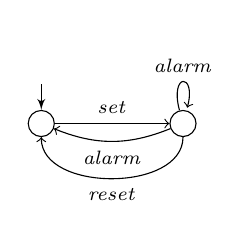
\begin{tikzpicture}[font=\sffamily\scriptsize]
      \node[vertex] (a) at (0, 0) {};
      \node[vertex] (b) at (1.8, 0) {};
      \node at (0, 1.1) {};

      \draw[edge] (0, 0.5) to (a);
      \path[->] (a) edge  node[above] {$\mathit{set}$} (b);
      \path[->] (b) edge  [bend left=22] node[below] {$\mathit{alarm}$} (a);
      \path[->] (b) edge  [loop above] node {$\mathit{alarm}$} ();
      \path[->] (b) edge  [bend left=90] node[below] {$\mathit{reset}$} (a);
    \end{tikzpicture}
  \end{center}

  \end{document}
